\section{Introduction: Distributed informations Systems, an Overview}


\subsection{Information System}

An information system is a \bf{software} that manages a \bf{model} of some aspect of the \bf{real world} within a (distributed) computer system for a given \bf{purpose}.
\\
\\
We can identify 3 types of real world aspect:
\begin{itemize}
	\item \bf{Physical phenomena:} measure the environment and create models of physical phenomena: meteorological IS, geo IS,...
	\item \bf{Social organization:} capture the roles, relationship activities, ... in social organization such as business and institutions.
	\item \bf{Human thought:} model human thought and reasoning processes. Capture the meaning of texts and other media, assess the importance and quality of information but also model human traits such as sentiments or opinion.
\end{itemize}

\subsubsection{Model}
Mathematical structure consisting of a set of:
\begin{itemize}
\item \bf{Constant} (or identifier)
\item \bf{Function} (or relation)
\item \bf{Axioms} (or constraint)
\end{itemize}
Example of model: a physical phenomena:

\begin{itemize}
\item Constant: coordinate values, temperature values
\item Function: T(x,y) $\rightarrow$ return temperature for a given coordinate.
\item Axiom: $-60 < T(x,y) < 60$
\end{itemize}
A function can be represented:

\begin{itemize}
\item Implicitly: $f(x) = x^2$
\item Explicitly: $f(1) = 1, f(2) = 4, f(3) = 9$ also called \bf{data}
\end{itemize}
Information system strongly emphasize \bf{explicit} representation, because many aspect of the world are not algorithmically defined: birthdate of a person. \bf{Implicit} representation play nevertheless an important role for queries, view, user definition functions
\\
\\
A model is linked by an \bf{interpretation or relationship} to the real world $\rightarrow$ maps every constant of the model to some real word object and the function preserve all relationship that occur in the real world. The interpretation relationship is \bf{homomorphic}. 

\begin{figure}[!h]
\begin{center}
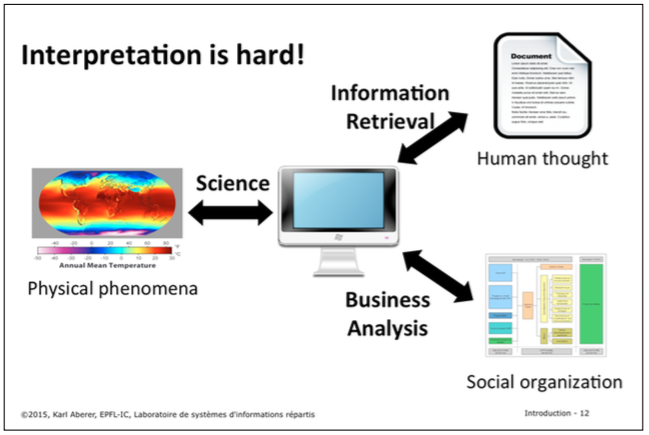
\includegraphics[scale=0.5]{figures/interpretation_hard.png}
\end{center}
\caption{interpretation is hard}
\end{figure}

Interpretation is hard because there is no way to formally verify function in the real world

\subsubsection{Data Management}
 \bf{Data model}: used to represent a model in a computer system. A data model D uses \bf{data structure} (associative array, labelled graphs, relational tables) and \bf{operation} (add(k,v), search(key),...) for the representation of the constants, data, and constraint of a model within a computer system.
 
 
 \paragraph{Database}: The collection of data represented in a data model D


\paragraph{Database Management System DBMS:} is a computer system designed to manage database. DBMS can be used to manage databases an this realize IS. The inverse is not necessarily true. 
\\
\\ Data Model is interchangeable used to represent two different things:

\begin{itemize}
	\item Data model used to represent a model within 	a computer system (sense we will use)	
	\item A formalism to specify a whole class of data model e.g; relational data model. Data modelling formalism consists of two part:
	
	\begin{itemize}
		\item \bf{Data definition model (DDL):} enables the specification of data models, consisting of possible data structure and integrity constraints. Specification of a data model using DDL is called \bf{database schema or schema}. Example \textit{CREATE TABLE student ... PRIMARY KEY}
		\item \bf{Data Manipulation language (DML):} allow to specify function in the data model. Ex: \textit{SELECT name FROM ...}
	\end{itemize}
\end{itemize}
Data Modelling formalism has 3 main component:

\begin{itemize}
	\item \bf{Data Structures:} collection of data structures which are used to represent database
	\item \bf{Integrity Constraints:} a language to express rules the data in database has to observe
	\item \bf{Manipulation:} a collection of operations which can be applied to the data structure to update, transform and query the data in the DB
\end{itemize}

\paragraph{Database Management System} is the software that implement a data modelling formalism ( MySql, PostgreSQL, Microsoft access, SQL Server, FileMaker, Oracle, but \bf{not} XML).

\paragraph{Logical Data Independence:} the same data can be viewed in different ways:
\begin{itemize}
	\item Views compute different data model on top of the same data stored in a database
	\item Corresponds to different model based on the same data (ex: university ranking, same data but each one find a different rank)
\end{itemize} 

\paragraph{Database Systems:} an IS based on a DBMS. The information system is concerned with providing a model for real world aspect, whereas the database system is concerned with the \bf{efficient management of the data structure required to represent the model}



\subsubsection{Data management Tasks}
2 challenges:
\begin{itemize}
	\item \bf{Efficient} management of large amounts of data (storage(column vs Row), indexing(B+- tree), search, aggregation)
	\item safety of the data: \bf{persistence } and \bf{consistency} of data under updates and failure (independent of lifetime of programs and type of failure)
\end{itemize}
Optimizing access to database:

\begin{itemize}
	\item \bf{Physical database design:} choice of the data structures and storage layout that match best the requirement of applications. Choice performed before the accesses to the database are executed
	\item \bf{Declarative Query Optimization:} choice of the best algorithm, given some storage and indexing scheme, when a concrete operation such as query is to be executed. Performed at the time the access to the database is executed
\end{itemize}
Transaction Management:

\begin{itemize}
	\item \bf{Isolation} others users do not influence own transaction
	\item System failure do not affect the execution of operations:
	\begin{itemize}
		\item \bf{Atomicity:} transaction are completely executed or not at all
		\item \bf{Durability:} once transactions are executed their results are never lost
	\end{itemize}
\end{itemize}

\paragraph{Physical Data Independence:}  concept that the same logical database ( having the same database schema) can be physically realized in many different way (using different physical database design) and the same logical operation (query, update) can be executed in physically different way using declarative query optimization and transaction management. 


\paragraph{Modeling architecture}: defined as standard by ANSI:
\begin{itemize}
	\item \bf{Conceptual Schema or Semantic layer:} Domain specific abstract models
	\item \bf{Logical Schema or semantic layer:} Data models
  	\item \bf{Physical Schema:} Physical storage on disk, in the network
\end{itemize}

\subsubsection{Information Management}
Between data and models:
\begin{itemize}
	\item \bf{Retrieval:} from models to data: given a model of reality we would like to learn about specifics aspect of reality
	\item \bf{Data mining:} from data to model: given a data find a model that match the data
\end{itemize}
Between model and real world:
\begin{itemize}
	\item \bf{Conceptual modeling:} From real world to Model: analyze the real world and specify a model
	\item \bf{Evaluation:} From model to real world: given a model evaluate it against reality.
\end{itemize}
Between data processing system and real world:
\begin{itemize}
	\item \bf{Control:} from data to real world: data generated can in the IS can be used to control real device
	\item \bf{Monitoring} from real world to data: the real world generate data that can be processed in the IS
\end{itemize}

\begin{figure}[!h]
\begin{center}
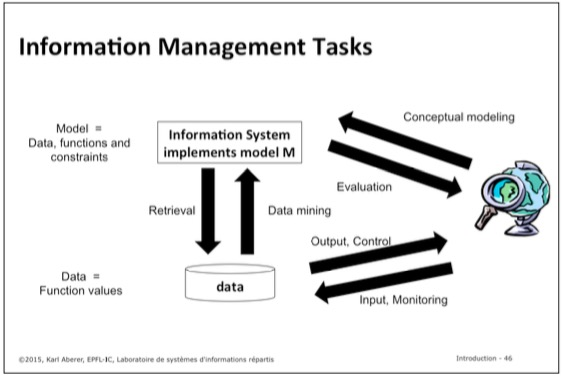
\includegraphics[scale=0.5]{figures/informationManagementTasks.jpg}
\end{center}
\caption{Information management tasks}
\end{figure}

\paragraph{Utility of information:} depend on:
\begin{itemize}
	\item \bf{Nature/Importance} of the decision
	\item \bf{Quality} of the decision
\end{itemize}

\begin{figure}[!h]
\begin{center}
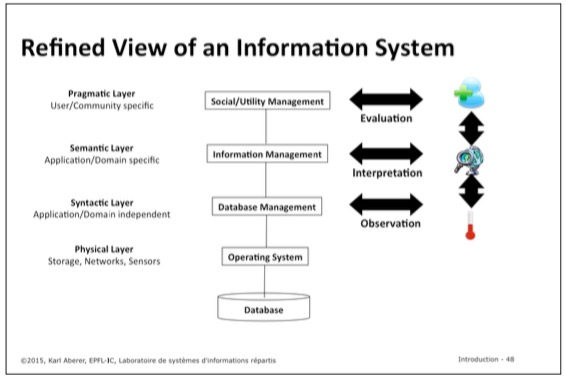
\includegraphics[scale=0.5]{figures/viewIS.jpg}
\end{center}
\caption{Overview of an information system}
\end{figure}

\subsection{Distributed information system}
\begin{itemize}
	\item \bf{Distributed data management:} use of distributed physical resources: locality of access, scalability, parallelism in the execution
	\item \bf{Heterogeneous information system:} use of different data models to represent the same information and different access methods. We have to deal with each IS are under the control of different \bf{Autonomous authorities:} $\Rightarrow$ independent users have to collaborate, coordinate, negotiate to perform information management task
\end{itemize}

\subsubsection{Distributed Data Management}
\begin{itemize}
\item \bf{Data Partitioning:} move the data to the nodes in the network where it is mostly used
\item \bf{Distributed Query Processing:}  deals with the problem of analysing queries and deciding which data can retrieved from which node
\item \bf{Data Replication:} replicate data if frequently used on different node $\oplus$ improves data access $\ominus$ update more expensive, consistency
\item \bf{Data Caching:} keep a copy of the data when transmitted in a network
\end{itemize}

\paragraph{Control:}
\begin{itemize}
\item \bf{Push access:} add new profile in database for example
\item \bf{Pull access:} query a specific profile for example
\end{itemize}


\paragraph{Communication model:}
\begin{itemize}
\item \bf{Unicast:} p2p connection
\item \bf{Multicast:} propagate requests to multiple receivers. example:\bf{Gossiping protocol:} sends request to local neighbourhood, then this neighbour spread the message,... until some peer can respond to the request
\item \bf{Broadcast:} send the request to all clients that are listening
\end{itemize}

\paragraph{Event:}
\begin{itemize}
\item \bf{Periodic:} periodic
\item \bf{Conditional:} on change(update)
\item \bf{Ad-hoc:} request by application or users (correspond to traditional client-server model)
\end{itemize}

\subsubsection{Heterogeneity}
\paragraph{Semantic heterogeneity:} the same real world aspect can be modelled differently. relating different models requires human intervention : human attention is a scare resource!

\paragraph{Solution: Mapping:}
\begin{itemize}
\item \bf{Standardization:} mapping through standard
\item \bf{Ontologies:} Mediated mapping. relate the model of an information system to a common model and use this mapping to construct a direct mapping among the different models used in the information systems\\
\item \bf{Mapping:} Direct mapping among two information system
\end{itemize}

\paragraph{Syntactic heterogeneity:} the same data can be represented using different data models (relational vs xml)

\begin{figure}[!h]
\begin{center}
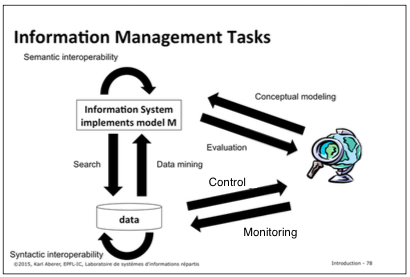
\includegraphics[scale=0.8]{figures/informationManagementTasks2.png}
\end{center}
\caption{Information management tasks}
\end{figure}


\subsubsection{The User Problem}
\begin{itemize}
\item bf{Trust:}Can I trust the information I received?
\item \bf{Privacy:} Can I trust the user to use my information I sent correctly
\end{itemize}
The \bf{more quality information} we reveal the \bf{more trust} we may expect, but the \bf{more} we also put out \bf{privacy} in danger.

One way to evaluate the quality of information, and thus the level of trust we can have in a user providing information, is to share recommendations with other users on how they perceive the quality of this information

\begin{figure}[!h]
\begin{center}
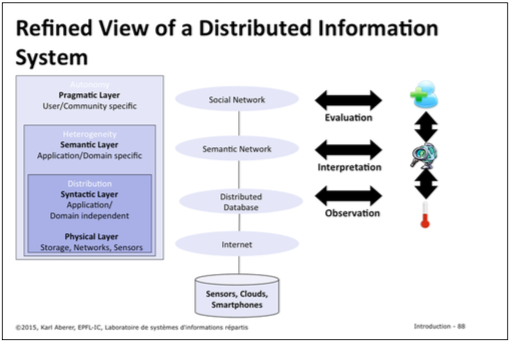
\includegraphics[scale=0.7]{figures/viewIS2.png}
\end{center}
\caption{Overview of an information system}
\end{figure}


